\documentclass[12pt, notitlepage, final]{article}

\newcommand{\name}{Vince Coghlan}

%\usepackage[dvips]{graphics,color}
\usepackage{amsfonts}
\usepackage{amssymb}
\usepackage{amsmath}
\usepackage{latexsym}
\usepackage{enumerate}
\usepackage{amsthm}
\usepackage{nccmath}
\usepackage{setspace}
\usepackage[pdftex]{graphicx}
\usepackage{epstopdf}
\usepackage[siunitx]{circuitikz}
\usepackage{tikz}
\usepackage{float}
\usepackage{cancel}
\usepackage{setspace}
\usepackage{overpic}
\usepackage{mathtools}
\usepackage{listings}
\usepackage{color}
\usepackage{qtree}
%\usepackage{gensymb}

\usetikzlibrary{calc}
\usetikzlibrary{matrix}
\usetikzlibrary{positioning}

%\numberwithin{equation}{section}
\newcommand{\dbr}[1]{d_{\mbox{#1BR}}}
\newtheorem{lemma}{Lemma}
\newtheorem*{corollary}{Corollary}
\newtheorem{theorem}{Theorem}
\newtheorem{proposition}{Proposition}
\theoremstyle{definition}
\newtheorem{define}{Definition}

\newdimen\digitwidth{}
\settowidth\digitwidth{0}
\def~{\hspace{\digitwidth}}

\setlength{\parskip}{1pc}
\setlength{\parindent}{0pt}
\setlength{\topmargin}{-3pc}
\setlength{\textheight}{9.0in}
\setlength{\oddsidemargin}{0pc}
\setlength{\evensidemargin}{0pc}
\setlength{\textwidth}{6.5in}

\DeclareMathOperator*{\argmin}{arg\,min}

%absolute value code
\DeclarePairedDelimiter\abs{\lvert}{\rvert}%
\DeclarePairedDelimiter\norm{\lVert}{\rVert}
\makeatletter
\let\oldabs\abs{}
\def\abs{\@ifstar{\oldabs}{\oldabs*}}
%
\let\oldnorm\norm{}
\def\norm{\@ifstar{\oldnorm}{\oldnorm*}}
\makeatother

\def\dbar{{\mathchar'26\mkern-12mu d}}
%\def \P[x]{\Frac{\partial}{\partial x}}
%\def \D[x]{\Frac{d}{dx}}
\newcommand{\PD}[2]{\frac{\partial#1}{\partial#2}}
\newcommand{\PF}[1]{\frac{\partial}{\partial#1}}
\newcommand{\DD}[2]{\frac{d#1}{d#2}}
\newcommand{\DF}[1]{\frac{d}{d#1}}
\newcommand{\fix}[2]{\left(#1\right)_#2}
\newcommand{\ket}[1]{|#1\rangle}
\newcommand{\bra}[1]{\langle#1|}
\newcommand{\braket}[2]{\langle{} #1 | #2 \rangle}
\newcommand{\bopk}[3]{\langle{} #1 | #2 | #3 \rangle}
\newcommand{\Choose}[2]{\displaystyle{} {#1 \choose{} #2}}
\newcommand{\proj}[1]{\ket{#1}\bra{#1}}
\def\del{\vec{\nabla}}
\newcommand{\avg}[1]{\langle#1\rangle}
\newcommand{\piecewise}[4]{\left\{\beginProtected{array}{rl}#1&:#2\\#3&:#4\endProtected{array}\right.}
\newcommand{\systeme}[2]{\left\{\beginProtected{array}{rl}#1\\#2\endProtected{array}\right.}
\def\Godel{G$\ddot{\mbox{o}}$del}

\title{Log-Linear Learning Over Large Iterations in Sudoku Puzzles}
\date{\today}
\author{\name}

\begin{document}

\maketitle

Sudoku is a puzzle game played on a $9\times9$ board.  The goal is to have a unique occurence
of each didget in each row, column, and $3\times3$ square.  This can be modeled as a game with the
following parameters:
\begin{itemize}
  \item{Players $N=\{1,2,\ldots,n\}$ Where $n$ is the number of empty spaces}
  \item{Actions $a_i\in\mathcal{A}$ where an action is a number between 1 and 9 and the actions set $\mathcal{A}=a_1\times a_2\times\cdots\times a_n$}
  \item{Utility Functions $u_i:\mathcal{A}\rightarrow \mathbb{R}$ Where the utility will be the number of repetitions of a
    player's current action in a row, column, or square.}
    \begin{equation} \label{util}
      u_i(a)=u_\text{row$_i$}(a)+u_\text{column$_i$}(a)+u_\text{square$_i$}(a)
    \end{equation}
    where
    \[
      u_\text{row$_i$} = \sum_{j\in i_{row}}(a_j=a_i)
    \]
  \item{Welfare Function $W(a):\mathcal{A}\rightarrow\mathbb{R}$ where the global welfare of an action represents the global
    desireability of that action.  Let $a$ be the joint action $(a_i, a_{-i})$ where $a_{-i}=(a_1,\ldots,a_{i-1},a_{i+1},\ldots,a_n)$}
\end{itemize}
We are given the ability to design the welfare function however we would like.  Suppose that our objective is captured
by a function $\phi:\mathcal{A}\rightarrow\mathbb{R}$ where
\begin{equation} \label{potgame}
  u_i(a_i,a_{-i}) - u_i(a_i^*, a_{-i}) = \phi(a_i, a_{-i})-\phi(a_i^*, a_{-i})
\end{equation}
A $\phi$ satisfying~\eqref{potgame} will be known as a potential function~\cite{shapley94}.  It can be shown that the
game of Sudoku has a potential function when we define the utility as in~\eqref{util}.  We begin by assuming that the
potential function will take the form
\[
  \phi(a)=\phi_\text{row}(a)+\phi_\text{column}(a)+\phi_\text{square}(a)
\]
We can then show that
\[
  \phi_\text{row}(a) - \phi_\text{row}(a^*) = u_\text{row$_i$}(a) - u_\text{row$_i$}(a^*)
\]
And so on.  When a player changes his number, he increases the amount of repetitions of that number by $1$.  By doing this,
however, he has unintentionally increased the amount of repetitions of any other player preforming the same action, and
decreased the amount of repetitions of his old action.  One would expect that the potential function is the sum of utilities
of each player
\[
  \phi_{\text{row}}(a) = \sum_{i\in N}u_{\text{row$_i$}}(a)
\]
\[
  \phi_{\text{row}}(a) - \phi_{\text{row}}(a^*) = \sum_{i\in N}u_\text{row$_i$}(a) - \sum_{i\in N}u_\text{row$_i$}(a^*)
\]
\[
 = \sum_{i\in N}\sum_{j\in i_{row}}(a_j=a_i) - \sum_{i\in N}\sum_{j\in i_{row}}(a_j=a^*_i)
\]
\[
 = \sum_{j\in i_{row}}(a_j=a_i) - \sum_{j\in i_{row}}(a_j=a_i) + \sum_{i\in N\backslash  \{i\}}\sum_{j\in i_{row}}(a_j=a_i) - \sum_{i\in N\backslash \{i\}}\sum_{j\in i_{row}}(a_j=a^*_i)
\]
Now we will use the fact that an increase in $n$ in the repetitions of $a_i$ corresponds to an increase of 1 of $n$
other players playing $a_i$.  This means that:
\[
 = \sum_{j\in i_{row}}(a_j=a_i) - \sum_{j\in i_{row}}(a_j=a_i) + \sum_{j\in i_{row}}(a_j=a_i) - \sum_{j\in i_{row}}(a_j=a_i)
\]
\[
 = 2(\sum_{j\in i_{row}}(a_j=a_i) - \sum_{j\in i_{row}}(a_j=a_i))
\]
This tells us that we have twice the potential function, meaning our potential function for the row is
\[
  \phi_{\text{row}}(a) = \frac{1}{2}\sum_{i\in N}u_{\text{row$_i$}}(a)
\]
This can be easily extended to squares and columns to find:
\begin{equation} \label{potfun}
  \phi(a) = \frac{1}{2}\sum_{i\in N}u_i(a)
\end{equation}

Since sudoku has a potential function, the minimization of the potential is a pure equilibrium~\cite{neyman97}.
Since we cannot have a negative potential by our definition of the utility, and a potential of 0 means that
there are no repetitions in any row, column, or square, a pure Nash Equilibrium exists, and must be the solution
of the puzzle.

We have half of our problem laid out, the next part is to define a learning algorithm that will converge to this
equilibrium.  Current strategies being studied currently include fictitious play~\cite{shapley96}, log-linear
learning~\cite{blume93}, and the cournot best reply process~\cite{cournot38} among others.  Many of these
learning algorithms converge to a Nash equilibrium~\cite{marden12}.  It has been shown~\cite{young93} that Log-linear
learning provides us the fact that, in any exact potential game, log-linear learning will induce a Markov chain with
a unique stationary distrobution $\pi \in \Delta(\mathcal{A})$ of the form
\begin{equation} \label{usd}
  \pi_a=\frac{e^{\frac{1}{T} \phi(a)}}{\sum_{\tilde{a}\in\mathcal{A}}e^{\frac{1}{T}\phi(\tilde{a})}}
\end{equation}
Since $\phi$ is zero at the solutions, we know that the distrobutions of the system as $T\rightarrow 0$ will be
distributed on solutions to the sudoku puzzle.  We can see this behavior for some simple sudoku puzzles, for example,
this puzzle was solved in 28836 iterations, with a temperature of $T=0.5$.

\begin{figure}[H]
\begin{center}
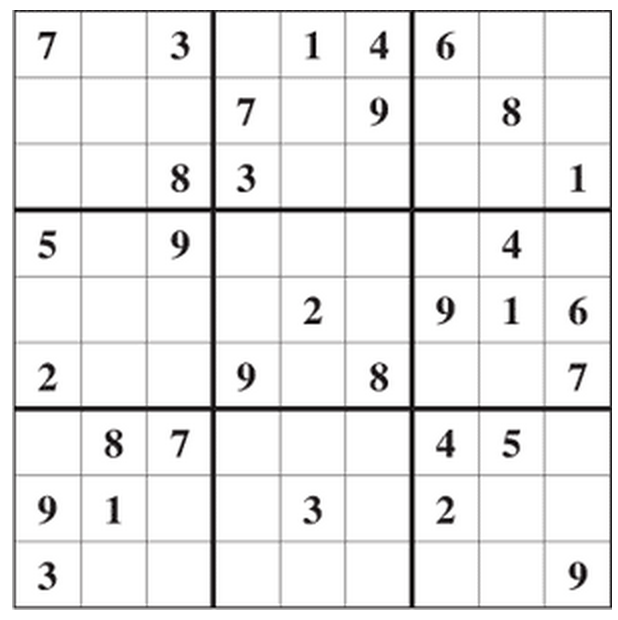
\includegraphics[width=5cm]{f1}
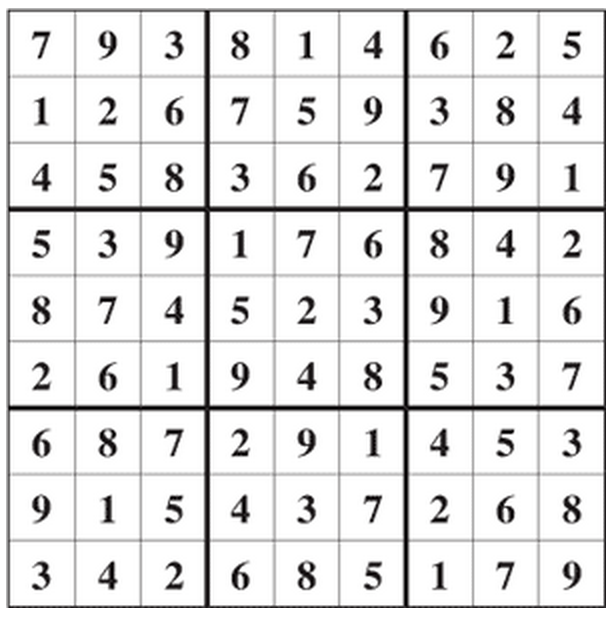
\includegraphics[width=5cm]{f2}
\end{center}
\end{figure}

The potential can be seen

\begin{figure}[H]
\begin{center}
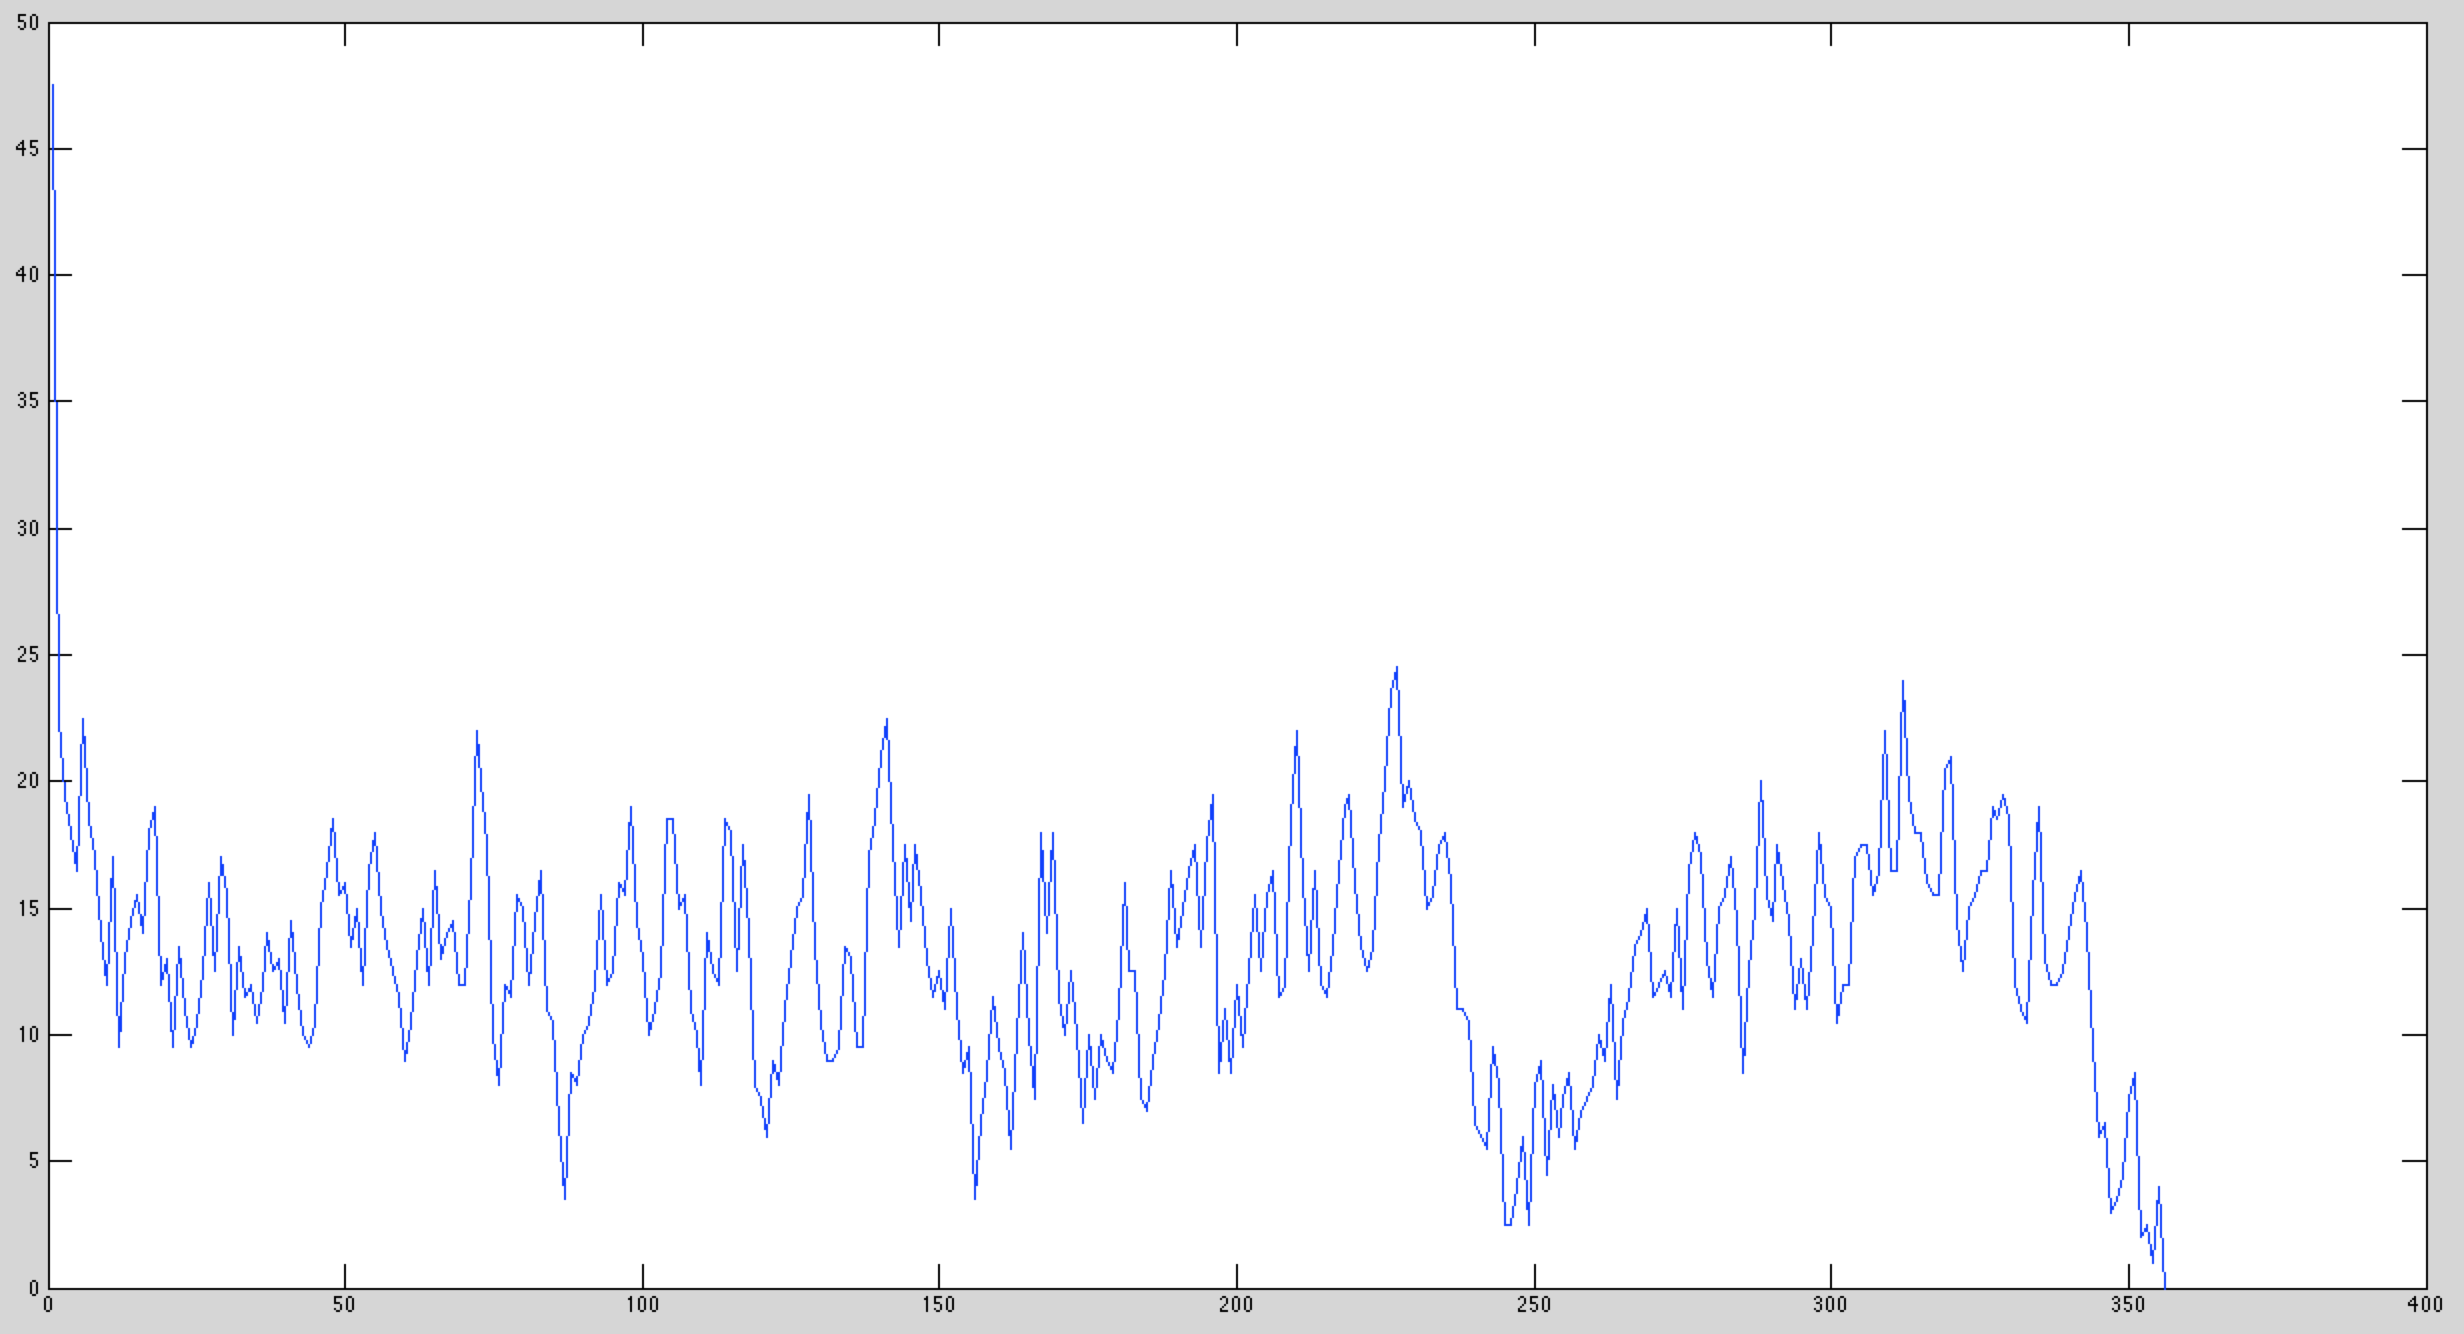
\includegraphics[width=12cm]{f3}
\end{center}
\end{figure}

You can see that once the potential is 0, we are done, and the puzzle is solved.  We can see a different story if
we run from a different initial condition.

\begin{figure}[H]
\begin{center}
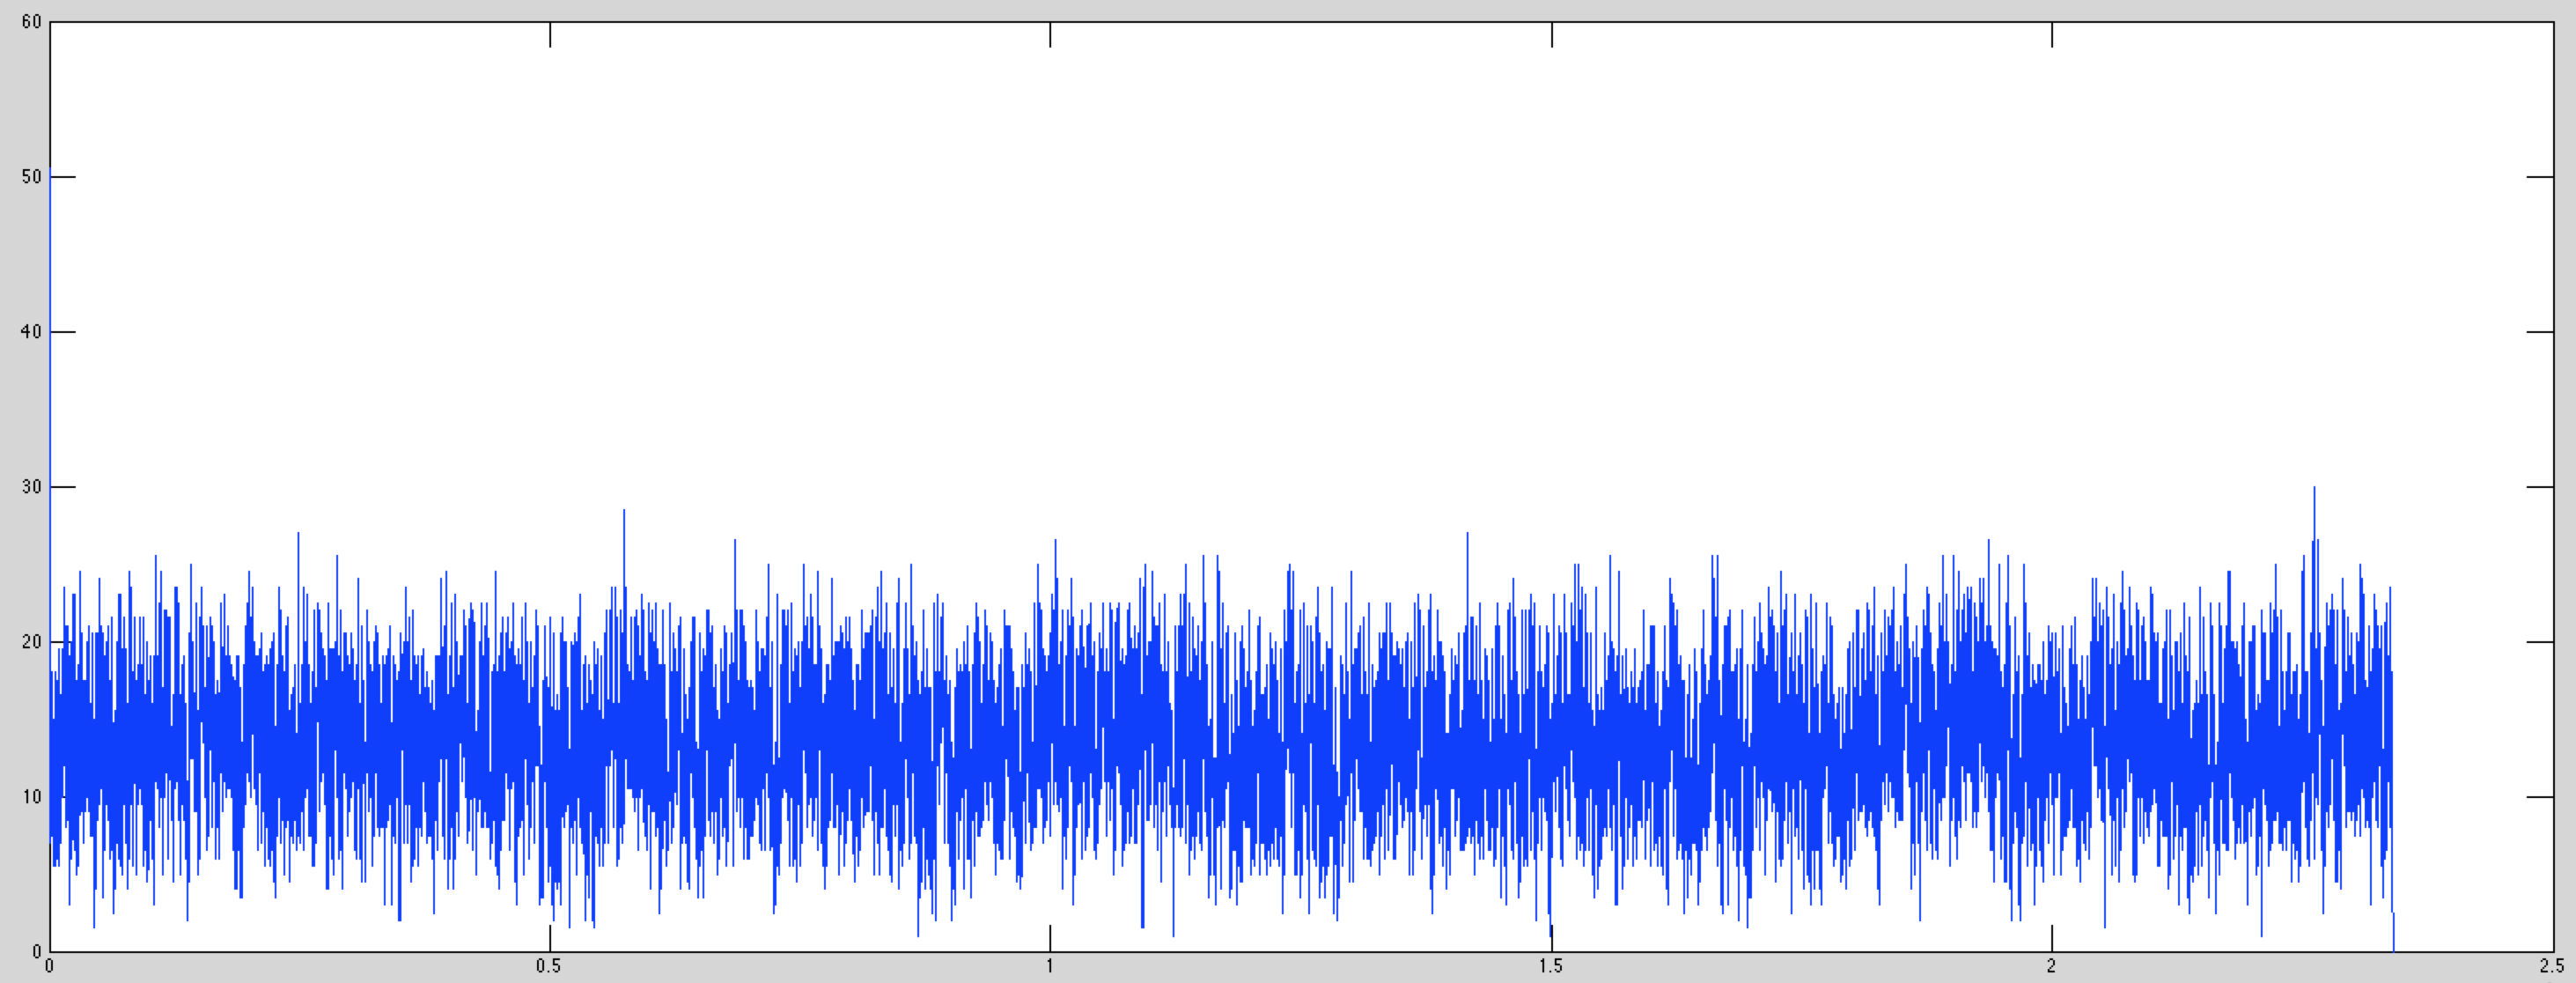
\includegraphics[width=12cm]{f4}
\end{center}
\end{figure}

When we start from a different initial condition, we get stuck in a puzzle configuration that is not bad, but not
a solution to the puzzle.  There is sufficiently high resistance between this state and the actual solution state
so that moving to the solution requires many iterations.  It took 500000+ iterations to solve, since we spend most
of out time in the following puzzle configuration:

\begin{figure}[H]
\begin{center}
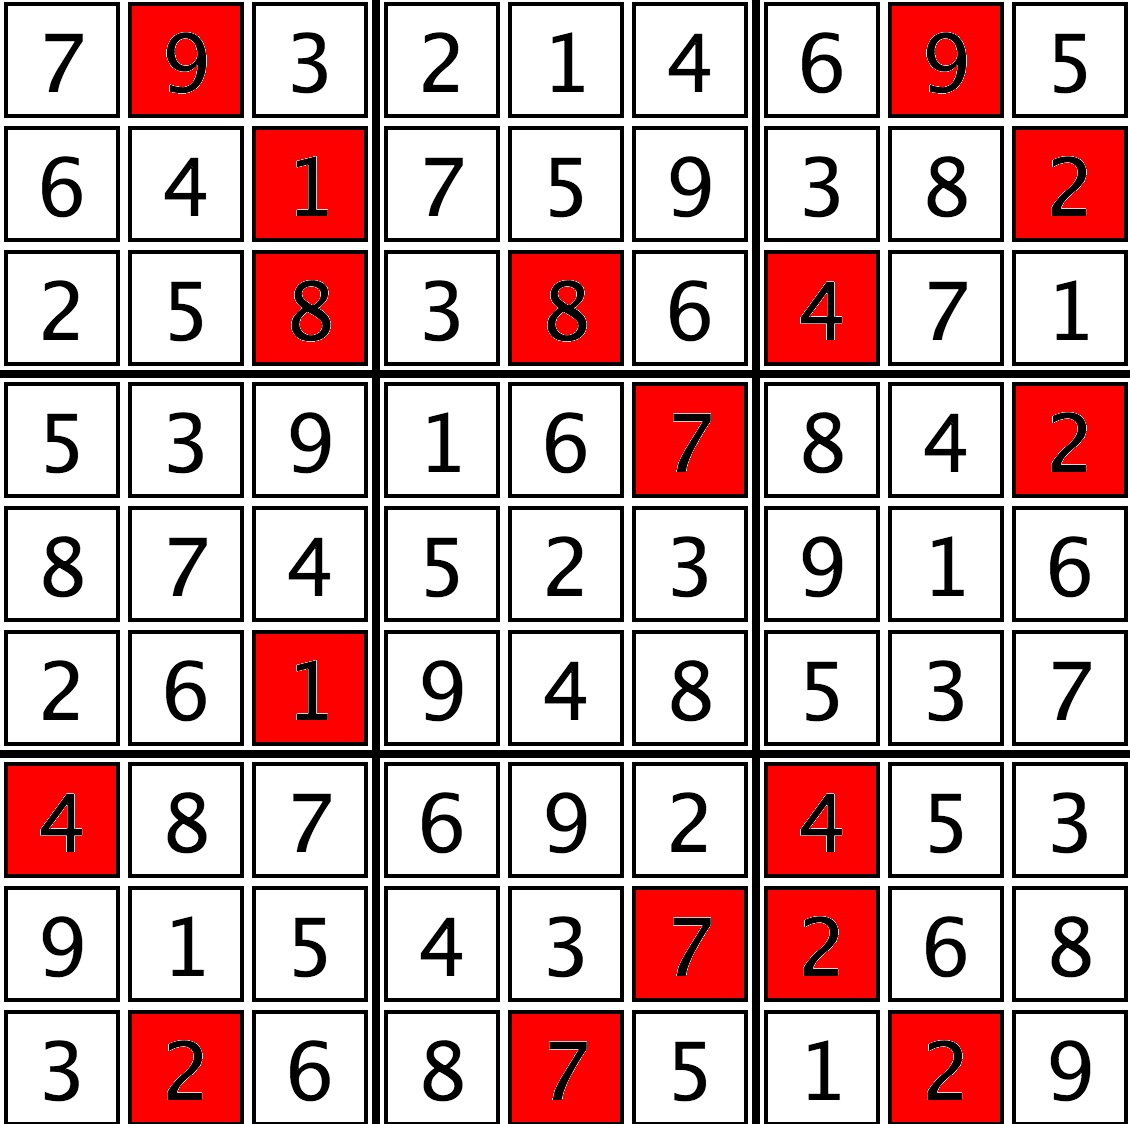
\includegraphics[width=7cm]{f5}
\end{center}
\end{figure}

Repeated numbers are highlighted in red.  You can see that this solution is close, with no more than one repitition
for any numbers.  If any of these repeated players chose to change their configuration, than they would either
maintain their cost, or increase it.  This fact means that it is sufficiently difficult to leave this
configuration, and requires many levels of $\epsilon$ to overcome.  It is clear from this that any learning method
will not do.  We need a learning method that has some sort of kickout probability so that we can leave an
innefficient Nash Equilibrium.  In the above case we are in equilibrium and staying there
wont solve the puzzle.  A learning algorithm like fictitious play or cournot adjustment process would remain at
this equilibrium.  This is where the value of log linear learning lies, the potential graph shows that we are constantly
in a state of finding a low potential solution, then leaving it to find another.  We can visualize what this would
look like in the following figure

\begin{figure}[H]
\begin{center}
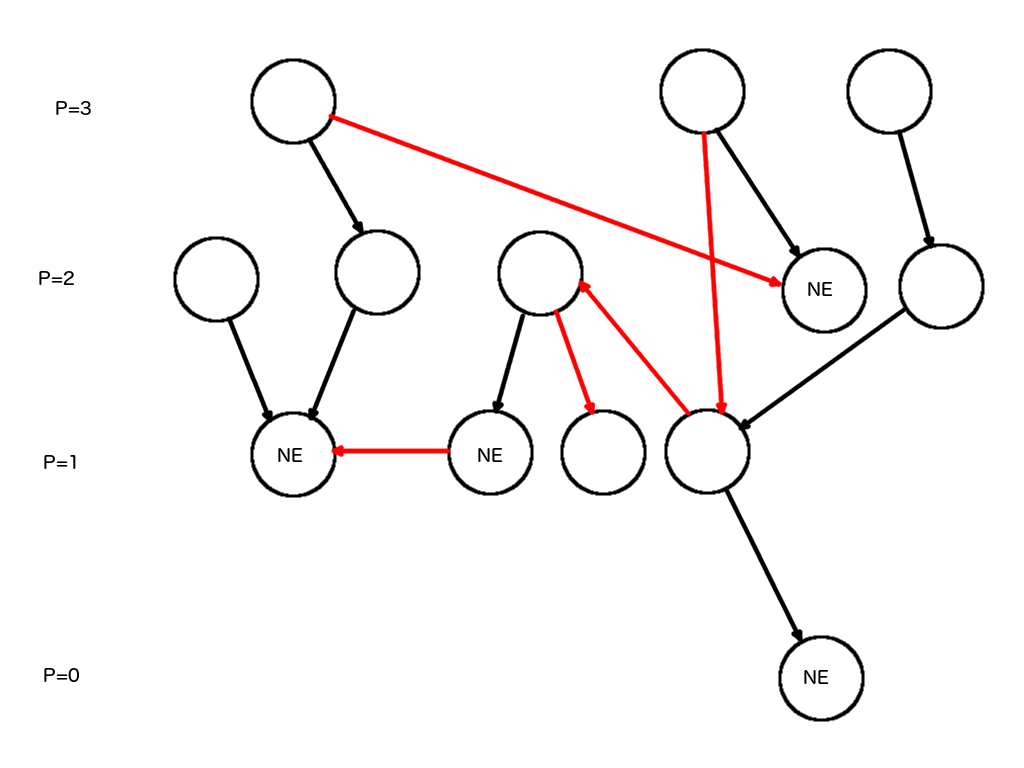
\includegraphics[width=12cm]{p1}
\end{center}
\end{figure}

Where the circles are states of the puzzle, each level of the picture is a level of potential.  There is only
one solution, meaning that there is only one configuration with potential of zero.  The black arrows are paths
of probability $1-\epsilon$ and the red arrows are paths of $\epsilon$.  In reality this graph extends to include
all possible configurations, a number as large as $10^{81}$.  The resistance between the left nash equilibrium
and the solution of the puzzle is 6 (note that any black arrow will have a red arrow going in the opposite
direction).  The resistance from the far right equilibrium would be 3.  This is what makes finding a solution
so difficult, and the reason why our learning algorithm needs a sort of ``kick-out'' probability that allows us
to leave a state.  If we increase the temperature to a higher value, say 2, we will more easily leave these
nodes, but the potential shows that we have too much chaos in the system

\begin{figure}[H]
\begin{center}
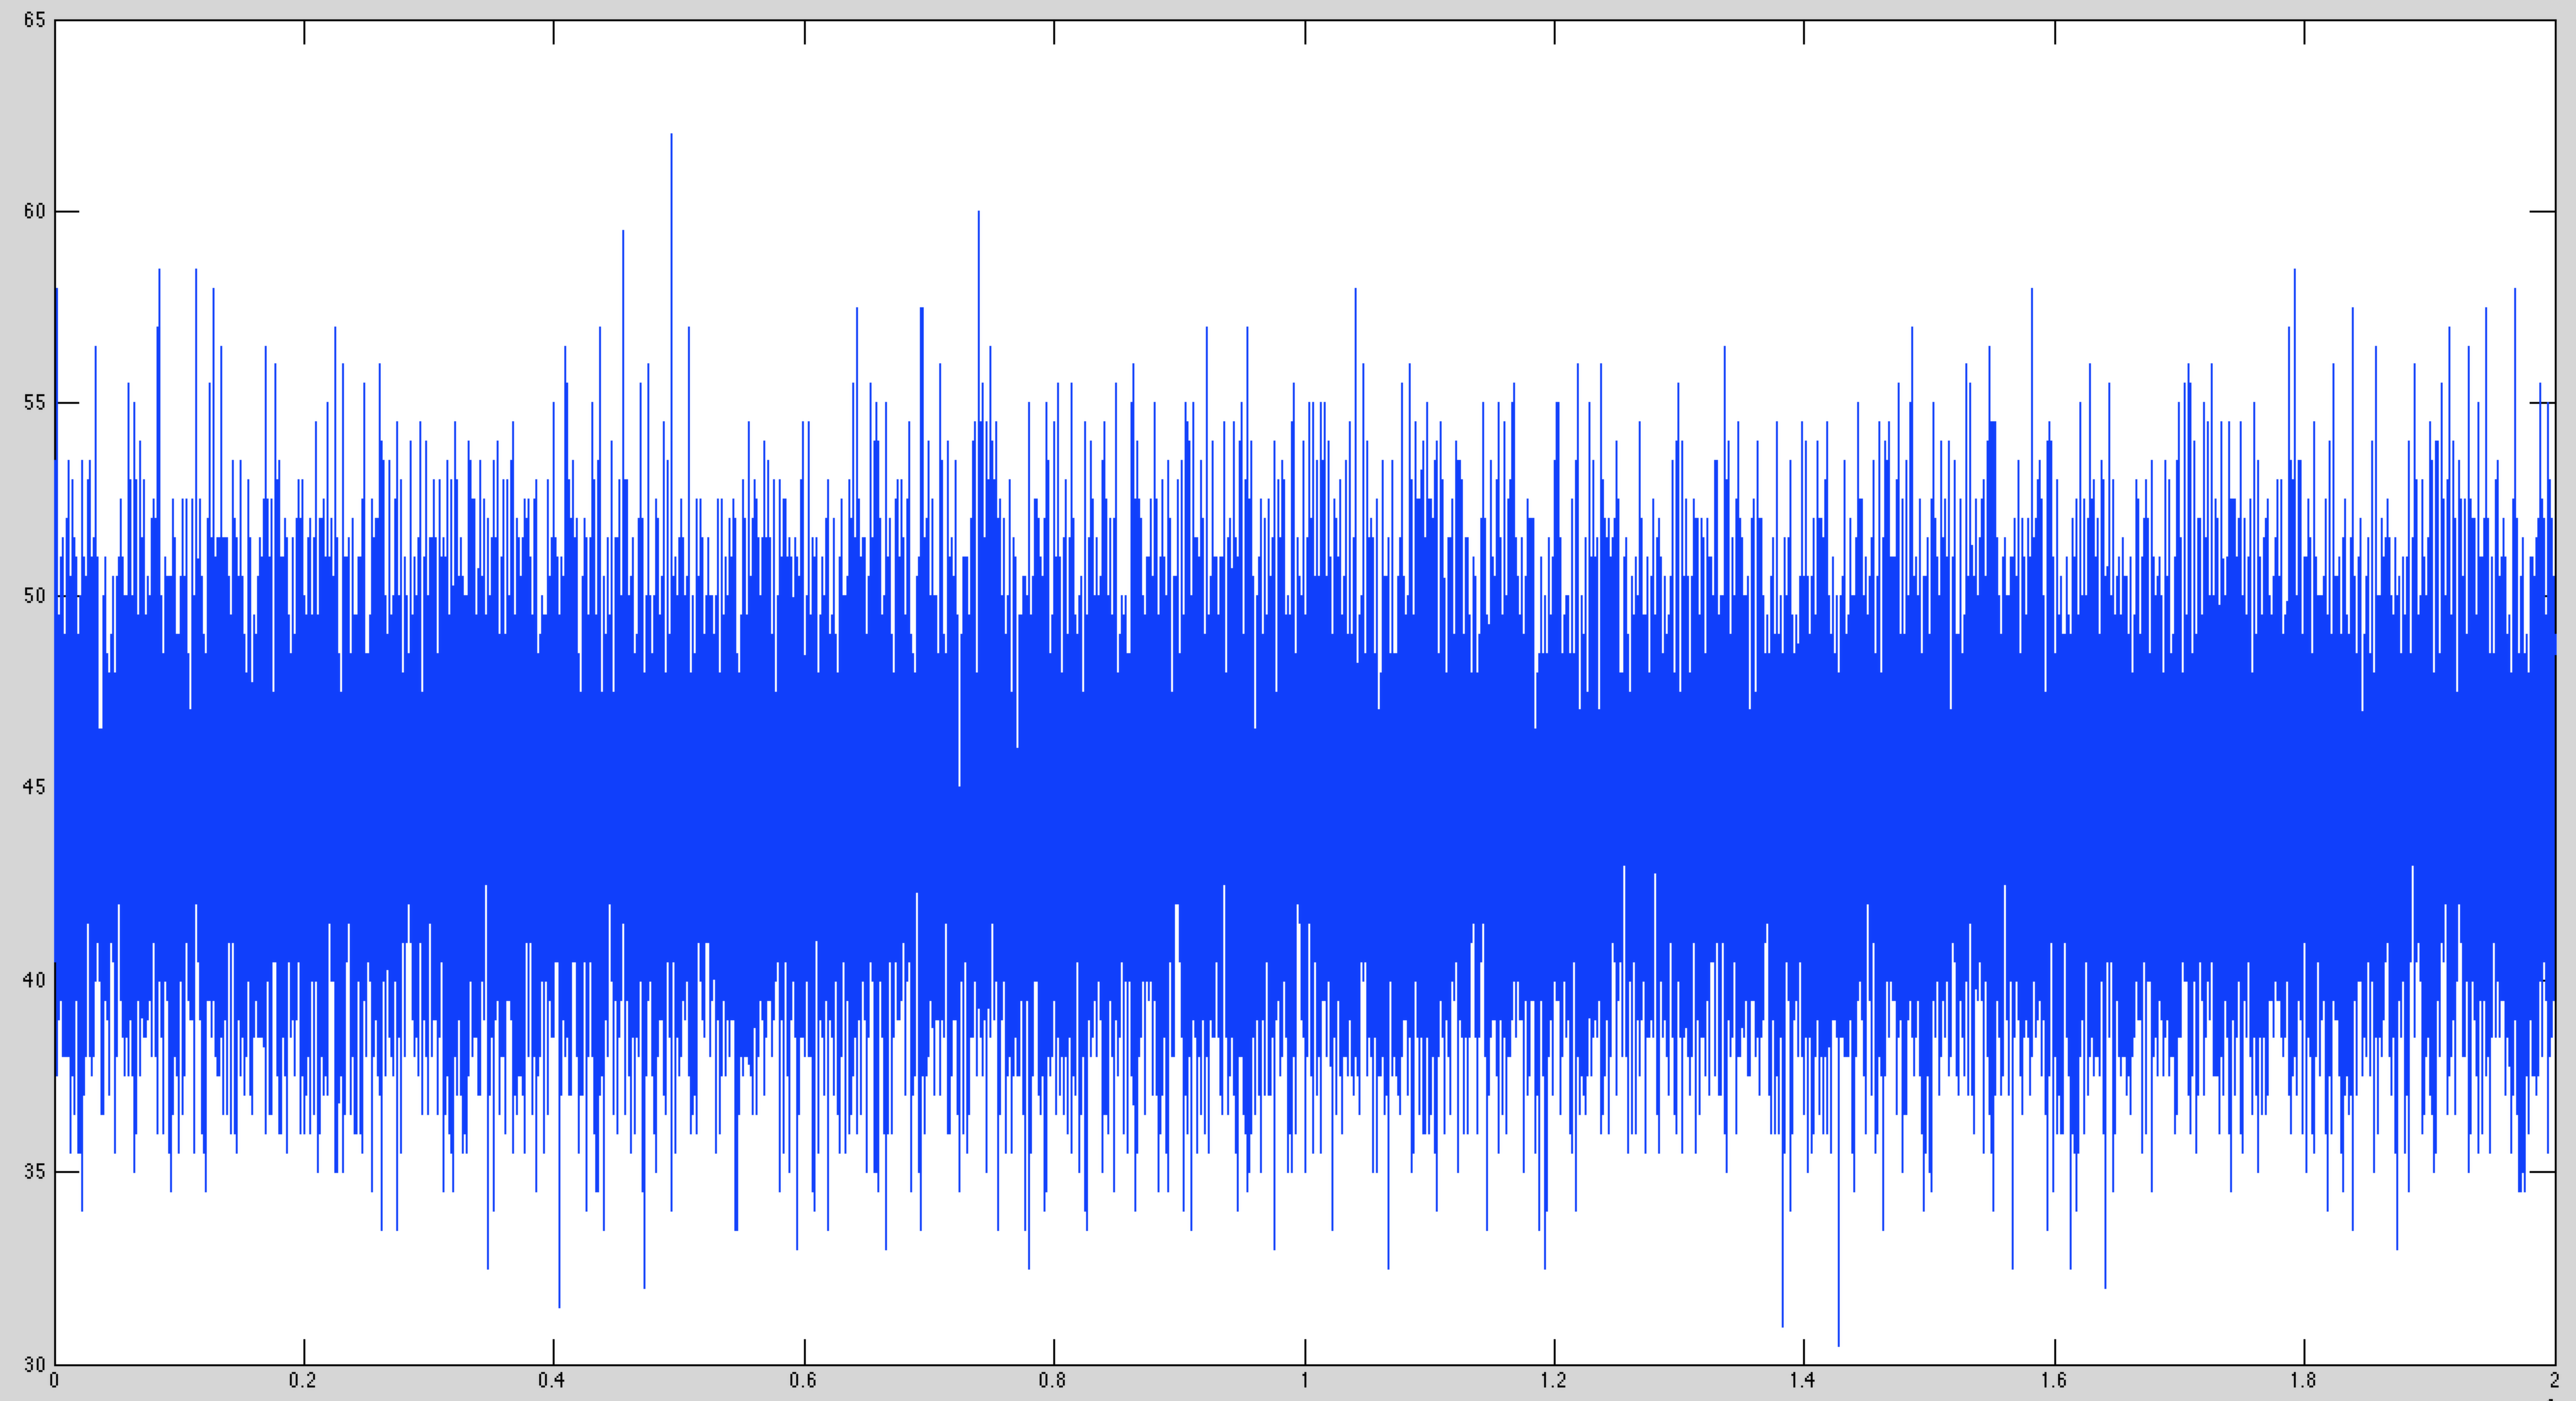
\includegraphics[width=12cm]{f6}
\end{center}
\end{figure}

This is not right, and wont find a solution in sufficient time.  You can see the potential arrive at values as low
as two, maybe these were on the correct path, but the large temperature forced these to go away from this
equilibrium.  A small temperature is no good either

\begin{figure}[H]
\begin{center}
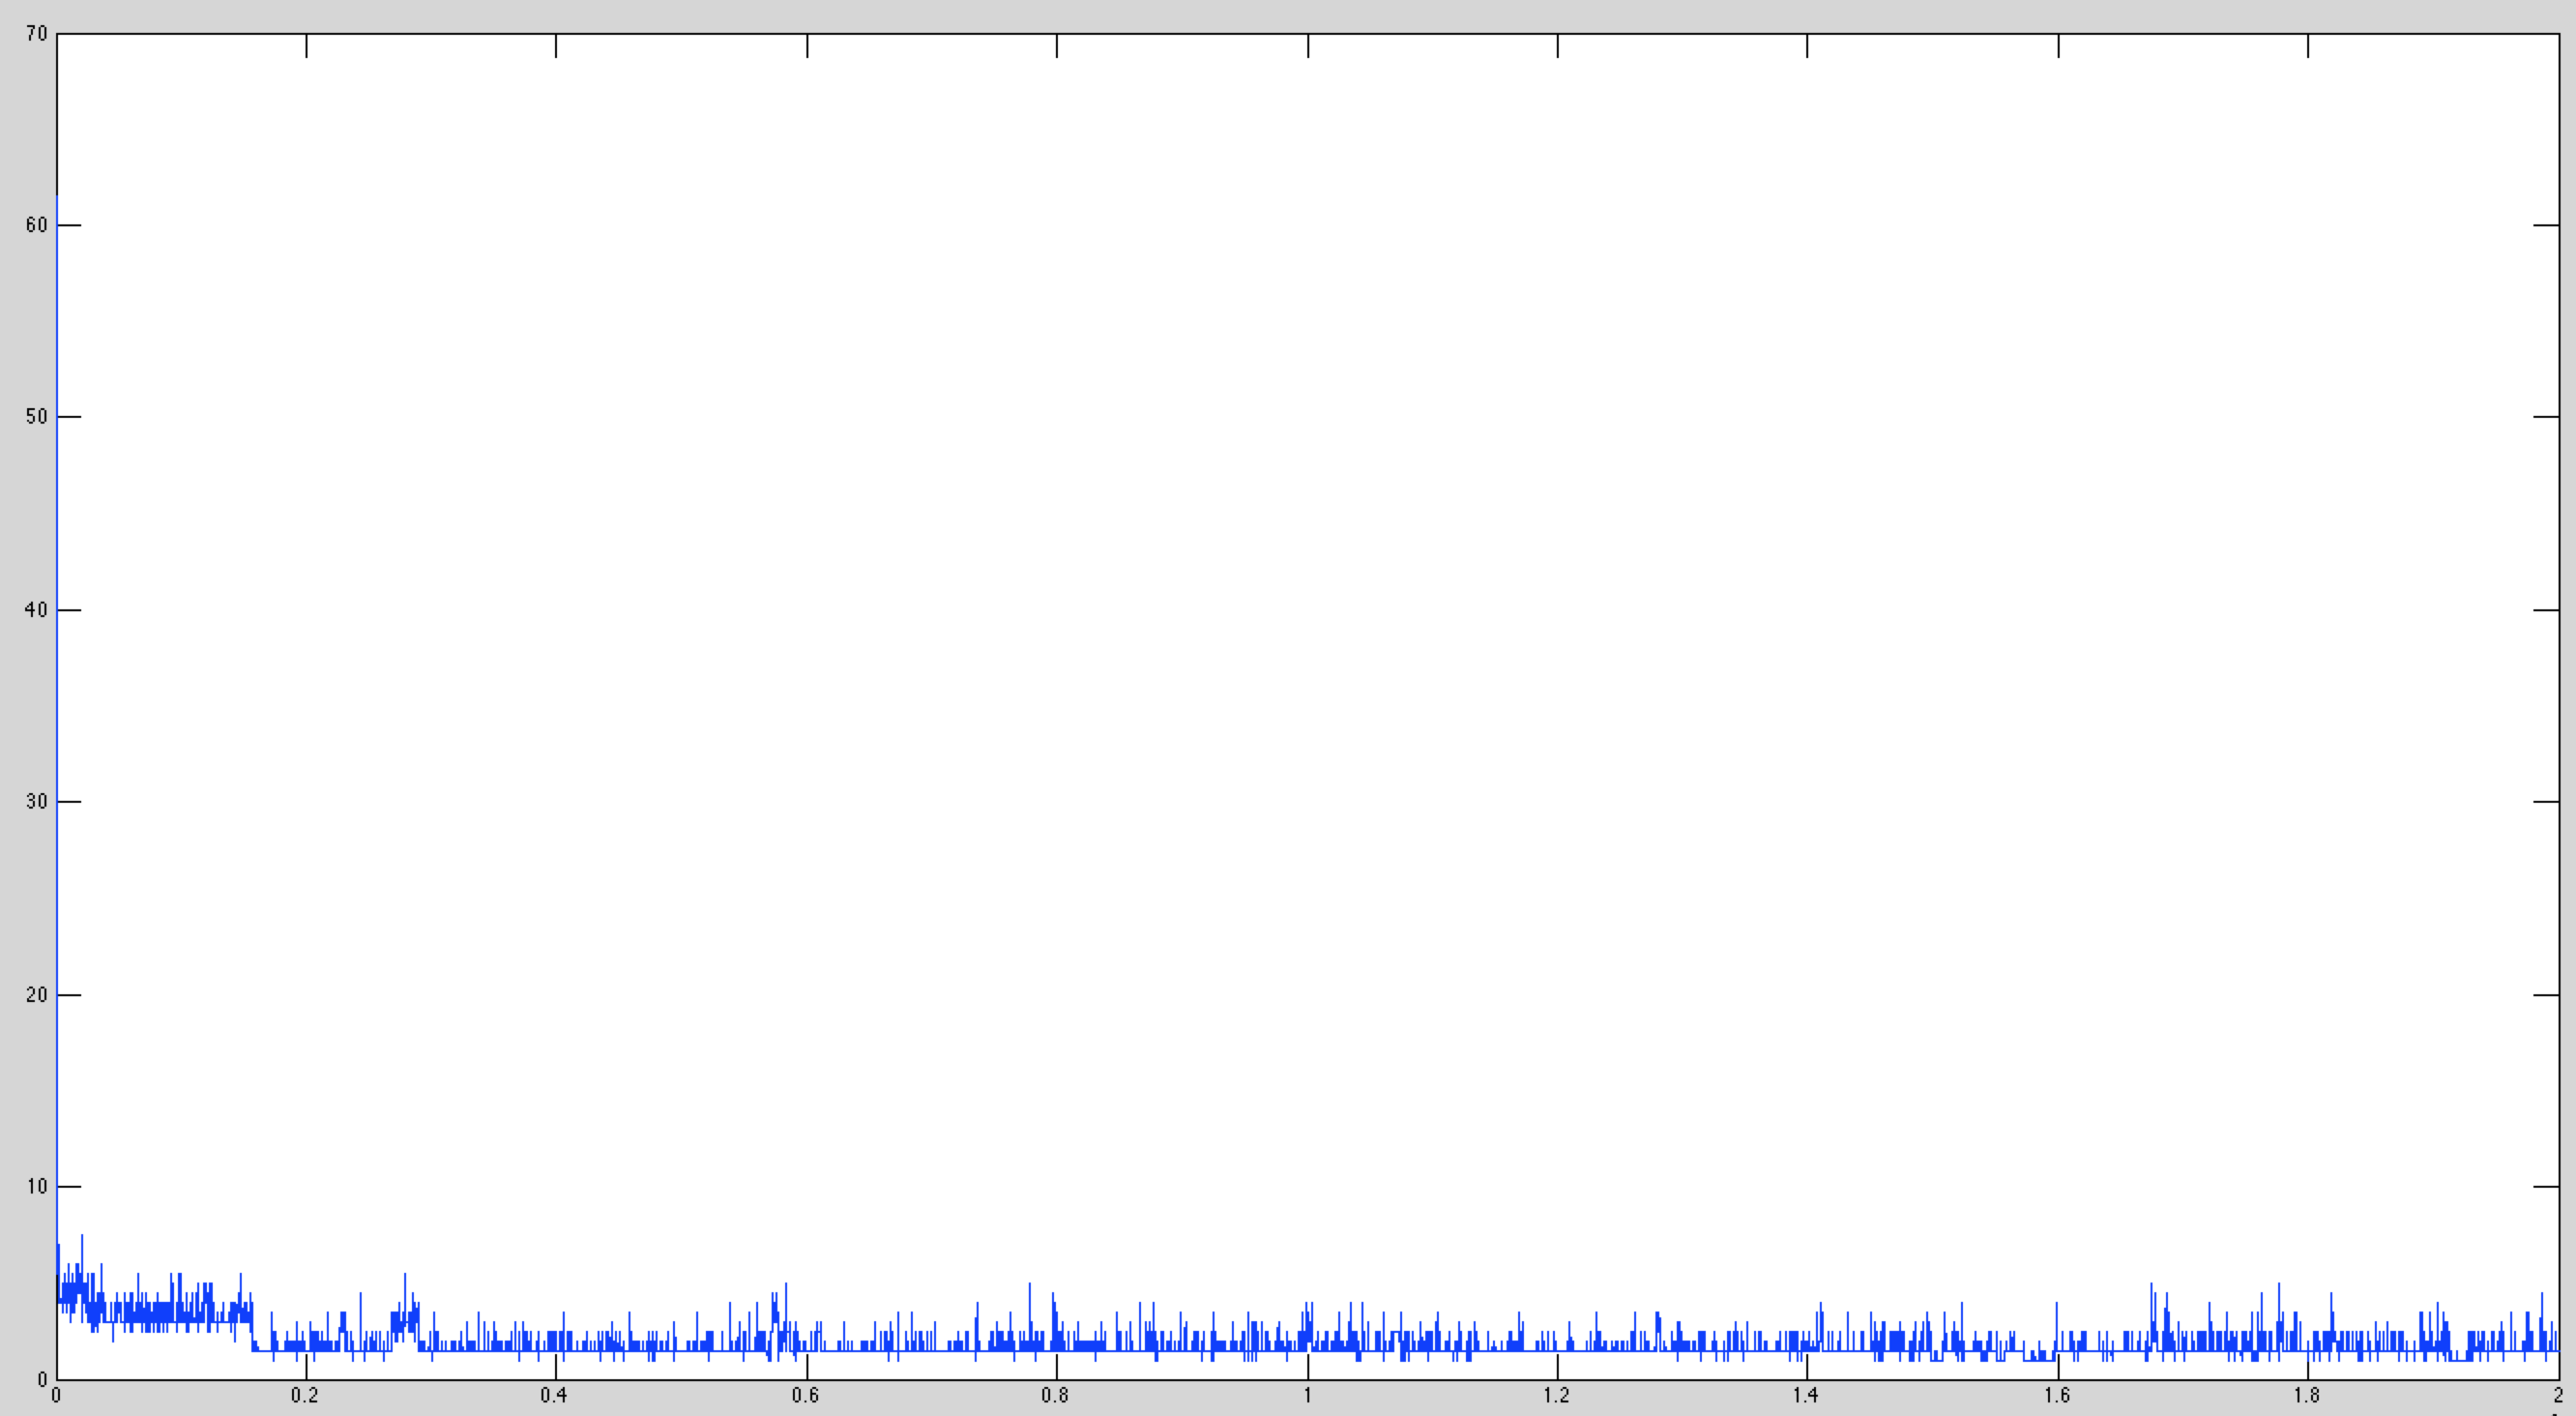
\includegraphics[width=12cm]{f7}
\end{center}
\end{figure}

We get stuck at another equilibrium.  There are, in fact, a multitude of equilibria, only one of which has a
potential of zero, the solution.  The probability epsilon becomes too small to solve this in a reasonable amount of
time.  We can see that these wont be solved in a reasonable time, but we know that in any exact potential game,
the only stochastically stable state is the potential minimizer~\cite{marden12}.  Games with multiple solutions
provide more insight into the problem at hand.  take for example~\cite{herzberg07}

\begin{figure}[H]
\begin{center}
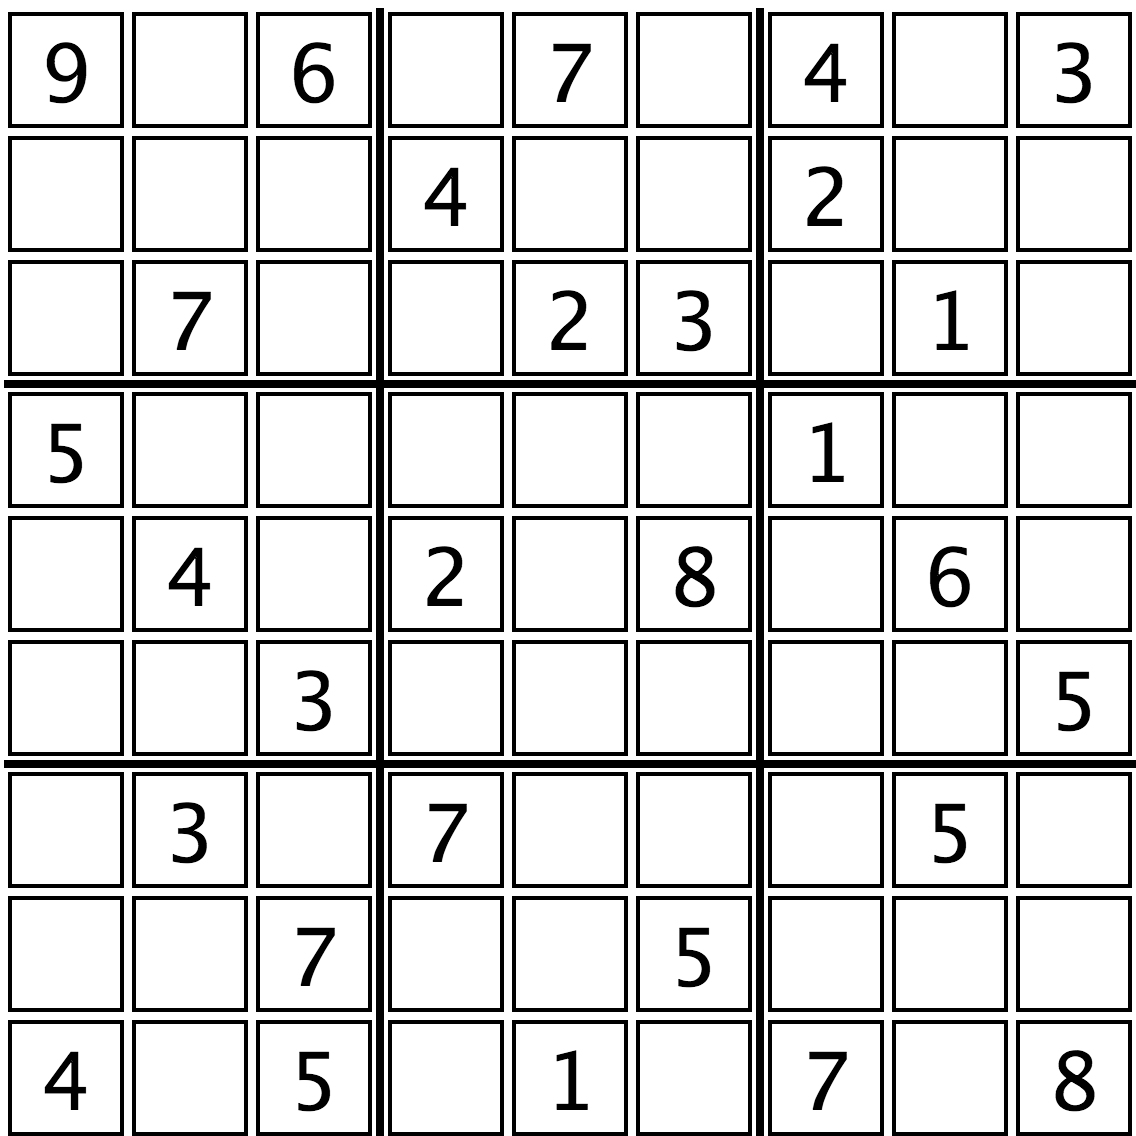
\includegraphics[width=5cm]{f8}
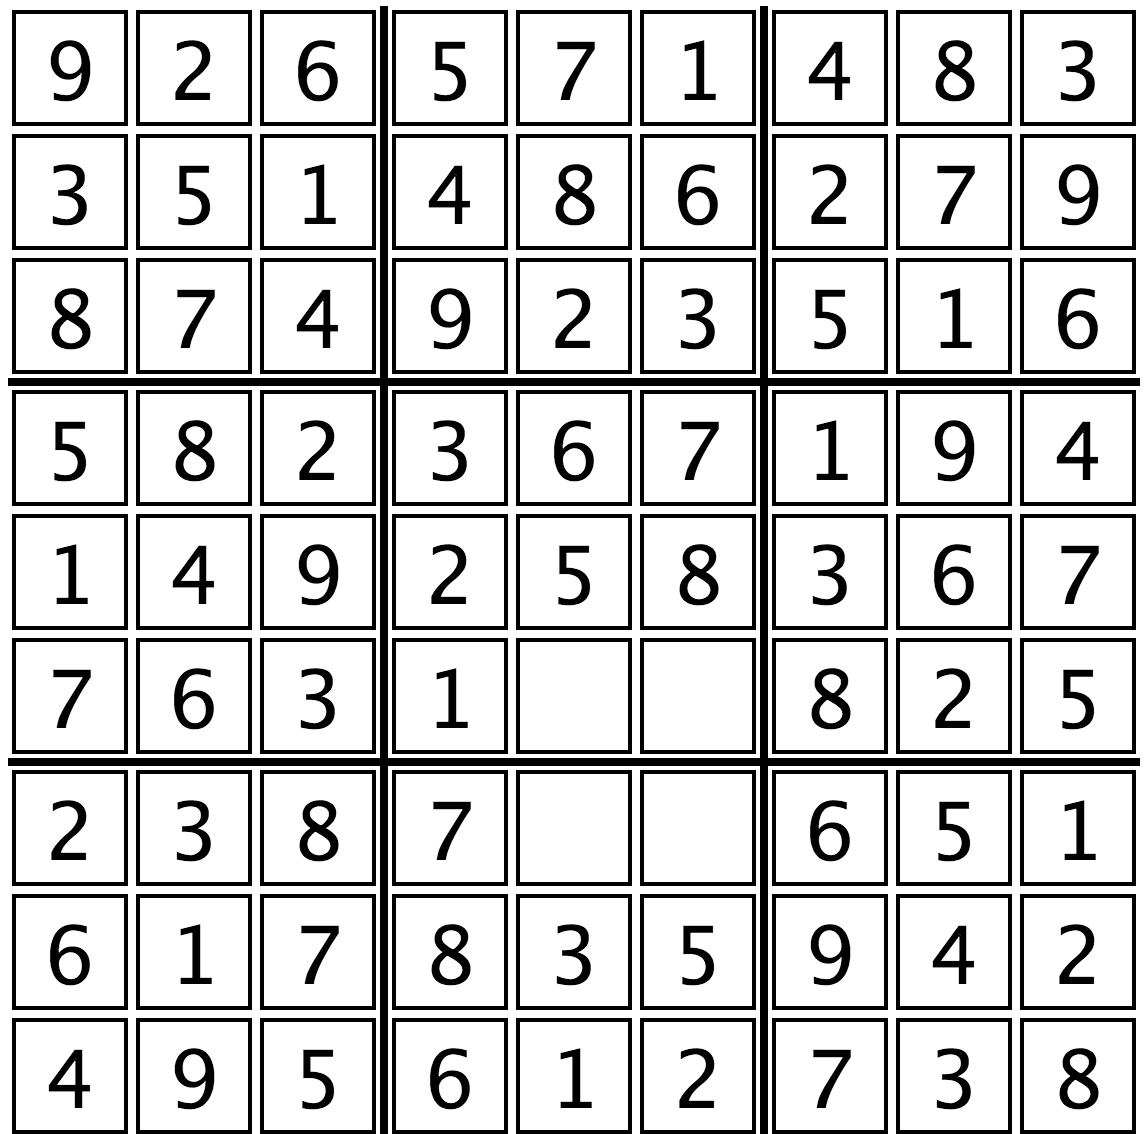
\includegraphics[width=5cm]{f9}
\end{center}
\end{figure}

The empty squares could be filled in with $\{9,4,4,9\}$ or $\{4,9,9,4\}$.  It can be show that any square of
the form $\{a,b,b,a\}$ in a puzzle can be reversed and another solution found~\cite{herzberg07}.  For
any of these cases, it will take a probability of $\epsilon$ to move to any other configuration, for example
$\{a, b, a, b\}$.  Once this change occurs, the probability of moving to one solution or the other becomes
a 50/50 chance, making the probability of changing equilibria to be $\epsilon/2$.  For sufficiently large
epsilon, it follows that the probability of landing in any particular solution in this situation would be
0.5.

What we need is a different algorithm that will prune the tree of posible states and possible equilibria.
This algorithm will take the current one and preform three simple modifications:
\begin{itemize}
  \item{The player making his move we be chosen from all players at random every iteration}
  \item{The player's possible actions will not include actions that are from initial set squares at
    the beginning of the game. i.e., all game states that are, by definition, not solutions will be
    eliminated from the possible future action profile of any player.}
  \item{The value of the temperature will vary over time, and will reset after sufficient iterations}
\end{itemize}

We can show that each of these maintains a potential game.  We will start from the bottom.  As long as
we keep our value of temperature "sufficiently large", then we will reach the same conclusion that we
do for regular log-linear learning, that is that the set of potential maximizers are the only
stochastically stable states.  This will force us out of a bad equilibrium if we are stuck there too long.
Next, if the player does not get to play any action he want, i.e., any action that started out on the
board to begin with, than the tree is trimmed of solutions we know dont exist.  Since the solution is not
included in that set, but is the stationary distrobution, than the rules of a potential game still apply.
If the player making the move has been chosed uniformly, than we can trust that we are still moving towards
a stationary distrobution, since each player is still updating asynchronously~\cite{ferrer10}.  It matters
not who updates in any given iteration, as long as someone does, and only one person does.  The solution
to the first puzzle we looked at can be seen followed by the potential function after finding it.

\begin{figure}[H]
\begin{center}
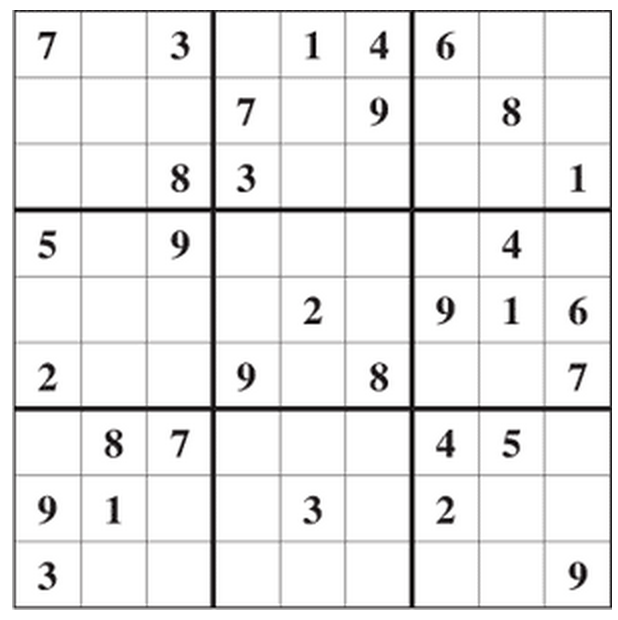
\includegraphics[width=5cm]{f1}
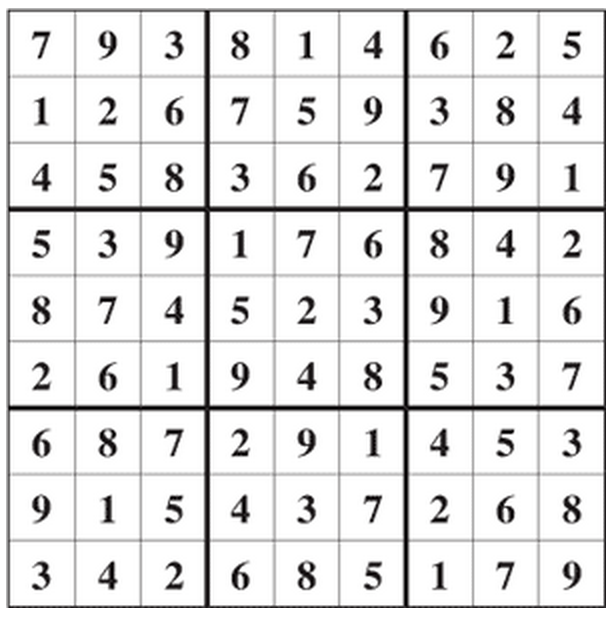
\includegraphics[width=5cm]{f2}
\end{center}
\end{figure}

\begin{figure}[H]
\begin{center}
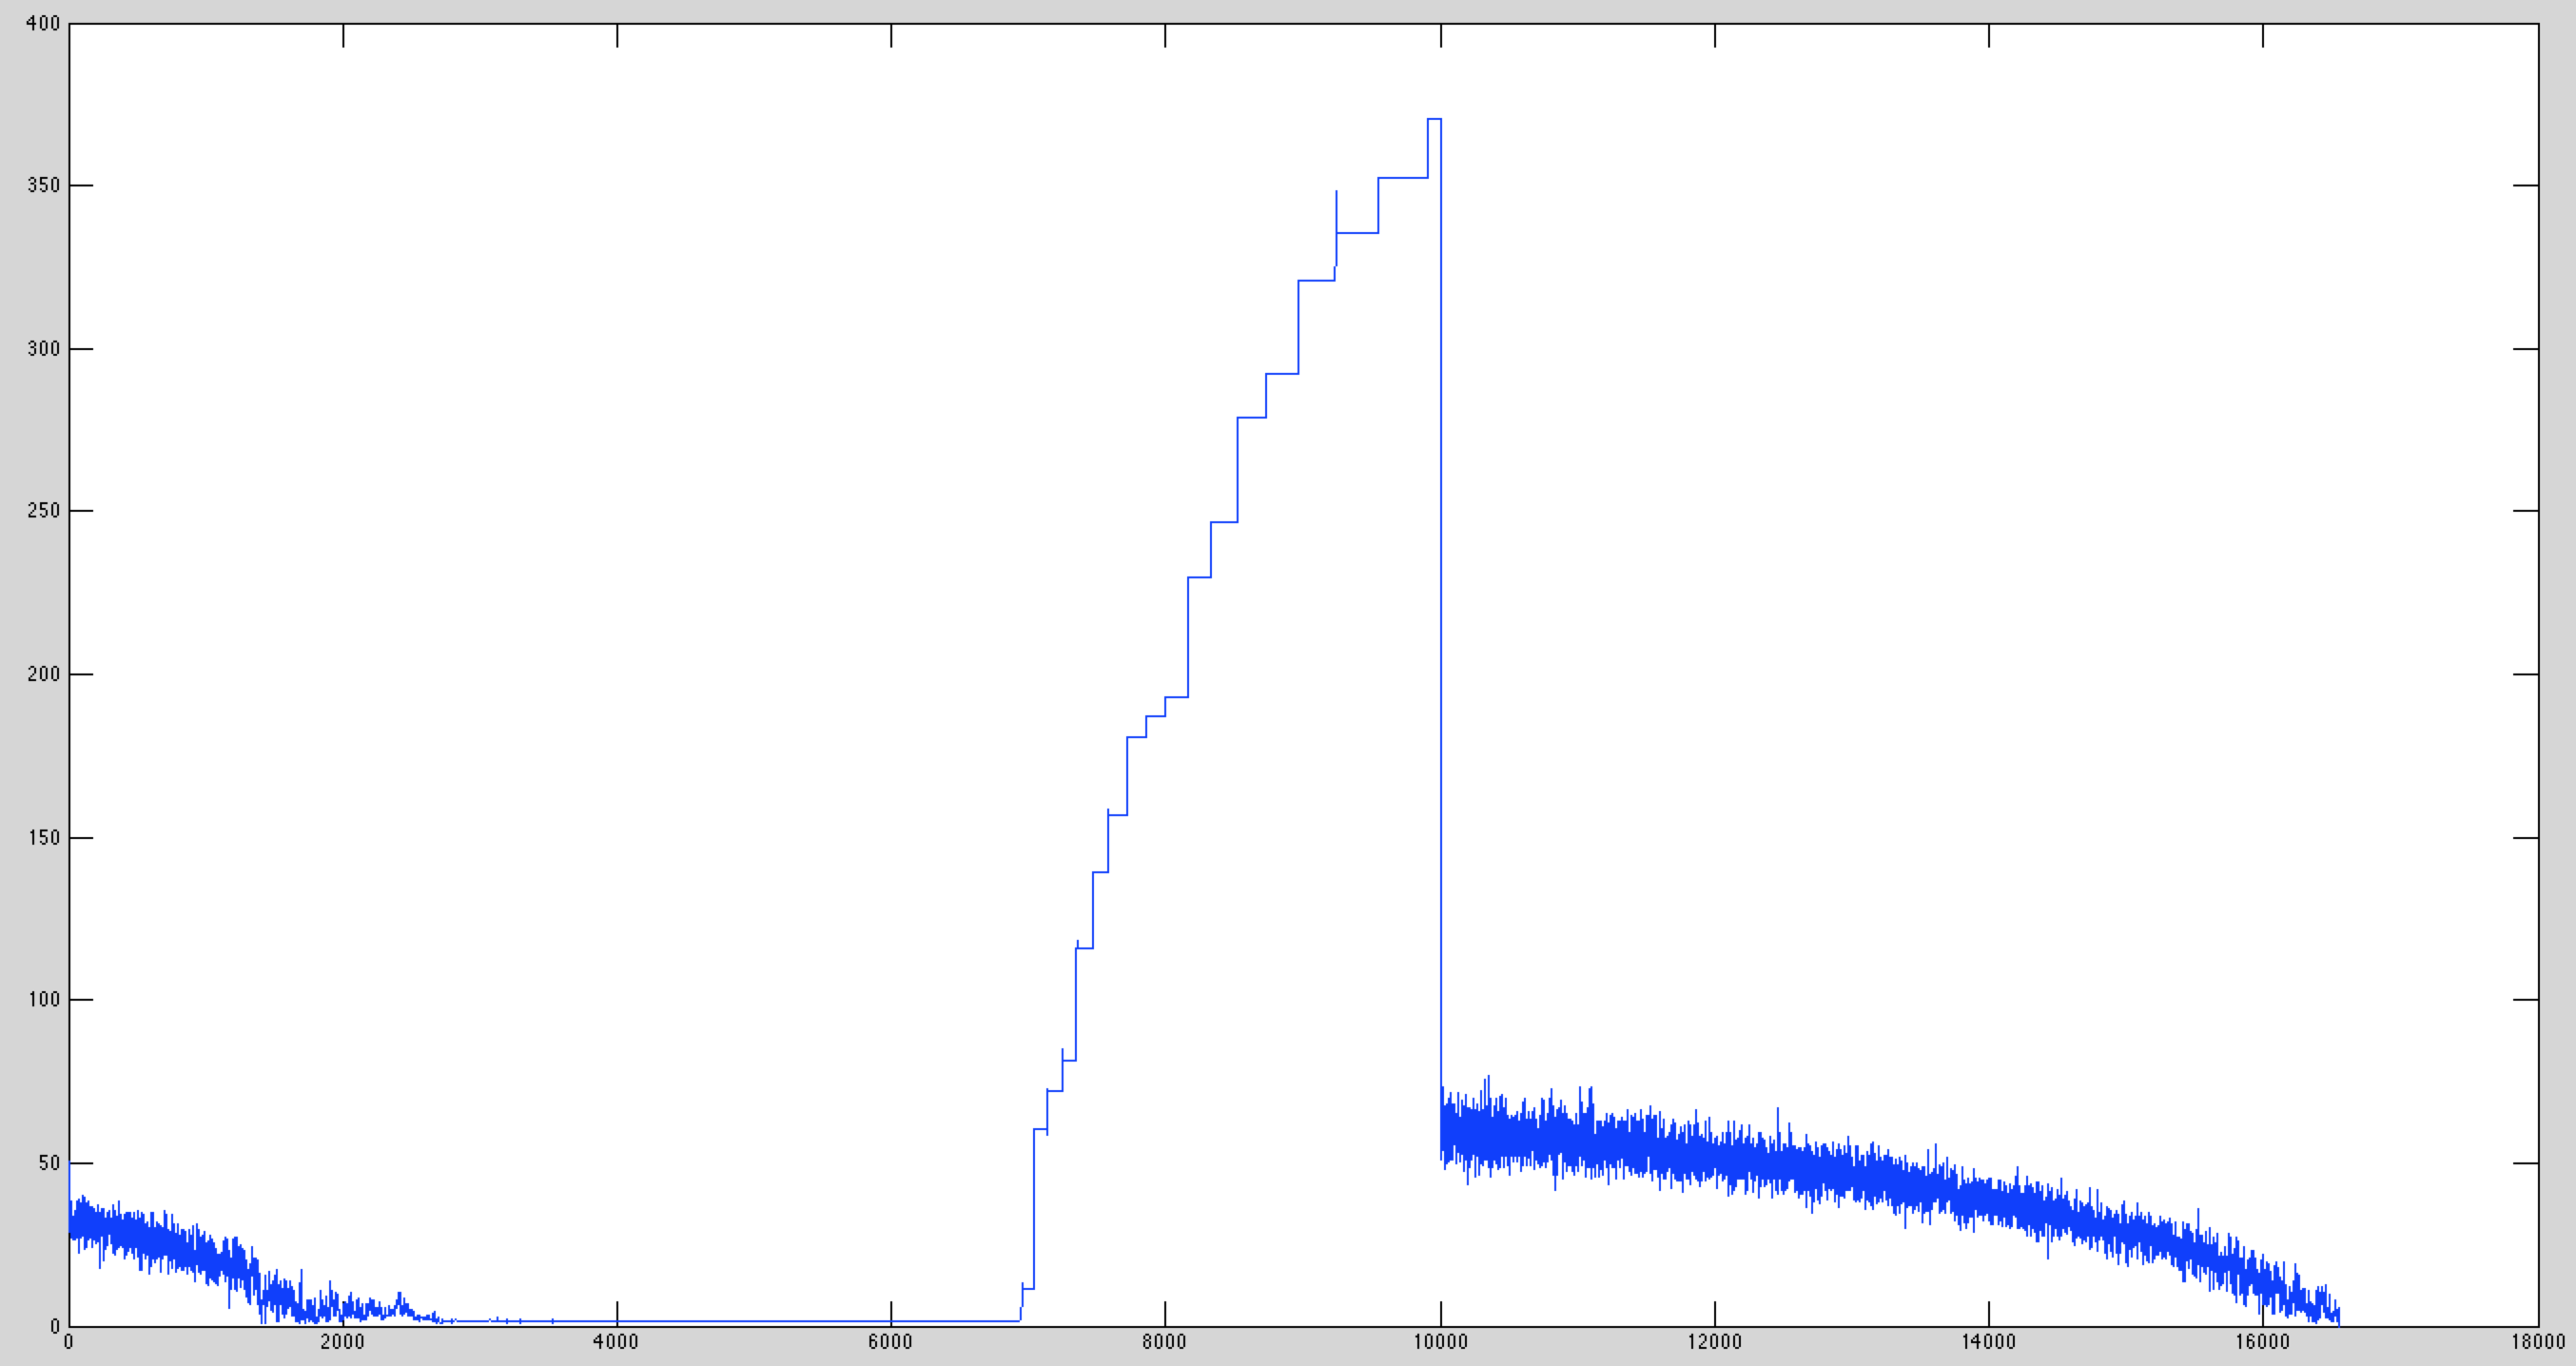
\includegraphics[width=12cm]{f10}
\end{center}
\end{figure}

Note that this is a very different graph.  In the previous graphs, we stay at around the same value, but never
get close to 0, in this graph, we decrease steadily as the temperature drops.  Once we reach a Nash equilibrium,
our temperature goes back to a chaotic value, and we try again.  This method finds a solution much faster and with
much higher reliability.  This is because we dont get stuck at a location with high resistance to the solution,
we instead move to a new state of the game that has a good chance of converging.

Finding an equilibrium in a real life engineering setting is not always possible with log-linear learning.
Sometimes we are forced to a nonoptimal equilibrium.  Constantly resetting the temperature allows us to
find a solution reliably fast.  Many of the puzzles ran did not converge under regular log-linear learning
in millions of iteration.  We know that it has to at some point, the math has proven that, but it is far more
efficient to change the temperature as a function of time.

\newpage
\begin{thebibliography}{9}

  \bibitem{ferrer10}
  C. Alos-Ferrer and N. Netzer,
  The logit-response dynamics.
  \emph{Ganes and Economic Behavior},
  68:413-427
  2010.

  \bibitem{blume93}
  L. Blume,
  The statistical mechanics of strategic interaction.
  \emph{Games and Economic Behavior},
  pp. 387--424,
  1993.

  \bibitem{cournot38}
  A. Cournot,
  \emph{Recherches sur les principes math\'{e}matiques de la th\'{e}orie des richesses},
  Hachette,
  1838.

  \bibitem{herzberg07}
  A. Herzberg and M. Murty,
  Sudoku Squares and Chromatic Polynomials.
  \emph{Notices of the AMS}
  June/July,
  2007

  \bibitem{neyman97}
  A. Neyman,
  Correlated Equilibrium and Potential Games.
  \emph{International Journal of Game Theory},
  pp. 223--227,
  1997.

  \bibitem{marden12}
  J. Marden and J. Shamma,
  Revisiting Log-Linear Learning: Asynchrony, Completeness and Payoff-Based Implementation
  \emph{Games and Economic Behavior},
  Volume 75, Issue 4, pp. 788--808,
  2012.

  \bibitem{shapley96}
  D. Monderer and L. Shapley,
  Fictitious Play Property for Games with Identical Interests.
  \emph{Journal of Economic Theory},
  Volume 68, pp. 258--265,
  1996

  \bibitem{shapley94}
  D. Monderer and L. Shapley,
  Potential Games.
  \emph{Games and Economic Behavior},
  Article No. 0044 pp. 124--143,
  1994.

\bibitem{young93}
  H.P. Young.
  The Evolution of Conventions.
  \emph{Econometrica},
  pp. 57--84,
  1993.


\end{thebibliography}

\end{document}
